\documentclass[a4paper,12pt]{article}
\usepackage[utf8]{inputenc}
\usepackage[spanish]{babel}
\usepackage{color}
\usepackage{parskip}
\usepackage{graphicx}
\usepackage{multirow}
\usepackage{listings}
\definecolor{mygreen}{rgb}{0,0.6,0}
\definecolor{lbcolor}{rgb}{0.9,0.9,0.9}
\DeclareGraphicsExtensions{.pdf,.png,.eps}
\usepackage{epstopdf}

\lstset{
backgroundcolor=\color{lbcolor},
    tabsize=4,    
%   rulecolor=,
    language=[GNU]C++,
        basicstyle=\scriptsize,
        aboveskip={1.5\baselineskip},
        columns=fixed,
        showstringspaces=false,
        extendedchars=false,
        breaklines=true,
        prebreak = \raisebox{0ex}[0ex][0ex]{\ensuremath{\hookleftarrow}},
        frame=single,
        numbers=left,
        showtabs=false,
        showspaces=false,
        showstringspaces=false,
        identifierstyle=\ttfamily,
        keywordstyle=\color[rgb]{0,0,1},
        commentstyle=\color[rgb]{0.026,0.112,0.095},
        stringstyle=\color{red},
        numberstyle=\color[rgb]{0.205, 0.142, 0.73},
%        \lstdefinestyle{C++}{language=C++,style=numbers}’.
}



\begin{document}

\begin{Large}
\textbf{Hecho por:} Christofer Fabián Chávez Carazas
\end{Large}

\section{Problema}

Codificar los siguientes autómatas por Diagrama de Transiciones y por Tabla de Transiciones:

\begin{itemize}

\item Autómata que verifique la correcta sintaxis de un identificador.
\item Autómate que verifique la correcta sintaxis de un número real.

\end{itemize}

\section{Código} 

\subsection{Funciones Adicionales}

Las funciones que se muestran a continuacíón son utilizadas para saber si un char constante o el contenido de un iterador de string, es un número o una letra.

\begin{lstlisting}

bool esNumero(const char &caracter){
    if(caracter >= 48 and caracter <= 57)return true;
    return false;
}

bool esLetra(const char &caracter){
    if(caracter >= 48 and caracter <= 57)return true;
    return false;
}

bool esNumero(string::iterator &letra){
    if(*letra >= 48 and *letra <= 57)return true;
    return false;
}

bool esLetra(string::iterator &letra){
    if(*letra >= 97 and *letra <= 122)return true;
    return false;}

\end{lstlisting}

\subsection{Verificar Identificador con Diagrama de Transiciones}

\begin{lstlisting}

void verificarIdentificador(){
    char letra;
    ifstream fe("datos.txt");
    int estado = 0;
    while(!fe.eof()){
        estado = 0;
        while(letra != ';' and !fe.eof()){
            fe>>letra;
            switch(estado){
                case 0:
                    if(letra >= 48 and letra <= 57){
                        estado = 2;
                    }
                    else if((letra >= 97 and letra <= 122) or letra == '_'){
                        estado = 1;
                    }
                    else{
                        estado = 2;
                    }
                    break;
                case 1:
                    if((letra >= 97 and letra <= 122) or (letra >=48 and letra <= 57) or letra == '_'){
                        estado = 1;
                    }
                    else if(letra == ';'){
                        estado = 3;
                    }
                    else{
                        estado = 2;
                    }
                    break;
            }
        }
        if(estado == 3){
            cout<<"Identificador correcto"<<endl;
       }
       else{
            cout<<"ERROR"<<endl;
       }
    fe>>letra;
    }
}
\end{lstlisting}

\subsection{Verificar Identificador con tabla de Transiciones}

\begin{lstlisting}
bool identificadorConTabla(){
    string frase;
    cin>>frase;
    int entrada;
    string::iterator letra = frase.begin();
    int estado = 0;
    int tabla[3][3] = {{2,1,-1},{-1,-1,-1},{2,2,10}};
    do{
        if(esLetra(letra) or *letra == '_'){
            entrada = 0;
        }
        else if(esNumero(letra)){
            entrada = 1;
        }
        else if(letra == frase.end()){
            entrada = 2;
        }
        else{
            return false;
        }
        estado = tabla[estado][entrada];
        if(estado == -1)return false;
        letra++;
    }while(estado != 10);
    return true;
}
\end{lstlisting}

\subsection{Verificar Número Real con Diagrama de Transiciones}

\begin{lstlisting}
bool numeroReal(){
    string frase;
    cin>>frase;
    int estado = 1;
    for(int i = 0; i < frase.size(); i++){
        switch(estado){
            case 1:
                if(esLetra(frase[i])){
                    estado = 2;
                }
                else{
                    return false;
                }
                break;
            case 2:
                if(esNumero(frase[i])){
                    estado = 2;
                }
                else if(frase[i] == '.'){
                    estado = 3;
                }
                else if(frase[i] == 'E'){
                    estado = 5;
                }
                else{
                    return false;
                }
                break;
            case 3:
                if(esNumero(frase[i])){
                    estado = 4;
                }
                else{
                    return  false;
                }
                break;
            case 4:
                if(esNumero(frase[i])){
                    estado = 4;
                }
                else if(frase[i] == 'E'){
                    estado = 5;
                }
                else{
                    return false;
                }
                break;
            case 5:
                if(esNumero(frase[i])){
                    estado = 7;
                }
                else if(frase[i] == '-' or frase[i] == '+'){
                    estado = 6;
                }
                else{
                    return false;
                }
                break;
            case 6:
                if(esNumero(frase[i])){
                    estado = 7;
                }
                else{
                    return false;
                }
                break;
            case 7:
                if(esNumero(frase[i])){
                    estado = 7;
                }
                else{
                    return false;
                }
                break;
        }
    }
    if(estado == 4 or estado == 7){
        return true;
    }
    return false;
}
\end{lstlisting}

\subsection{Verificar Número Real cond Tabla de Transiciones}


\begin{lstlisting}
bool numeroRealConTabla(){
    string frase;
    cin>>frase;
    int entrada;
    string::iterator letra = frase.begin();
    int estado = 1;
    int tabla[7][6] = {{2,-1,-1,-1,-1,-1},
                       {2, 3, 5,-1,-1,-1},
                       {4,-1,-1,-1,-1,-1},
                       {4,-1, 5,-1,-1,10},
                       {7,-1,-1, 6, 6,-1},
                       {7,-1,-1,-1,-1,-1},
                       {7,-1,-1,-1,-1,10}};
    do{
        if(esNumero(letra))
            entrada = 0;
        else if(letra == frase.end())
            entrada = 5;
        else{
            switch(*letra){
                case '.':entrada = 1;break;
                case 'E':entrada = 2;break;
                case '+':entrada = 3;break;
                case '-':entrada = 4;break;
                default: return false;
            }
        }
        estado = tabla[estado - 1][entrada];
        letra++;
        if(estado == -1)return false;
    }while(estado != 10);
    return true;
}

\end{lstlisting}

\section{Ejemplos}

\subsection{Verificar Identificador con Diagrama de Transiciones}

El archivo "datos.txt" tiene el siguiente contenido.

\begin{itemize}
\item temp;
\item temp1234;
\item 1234temp;
\item \_ 123;
\end{itemize}

\newpage

\begin{figure}[h]
\centering
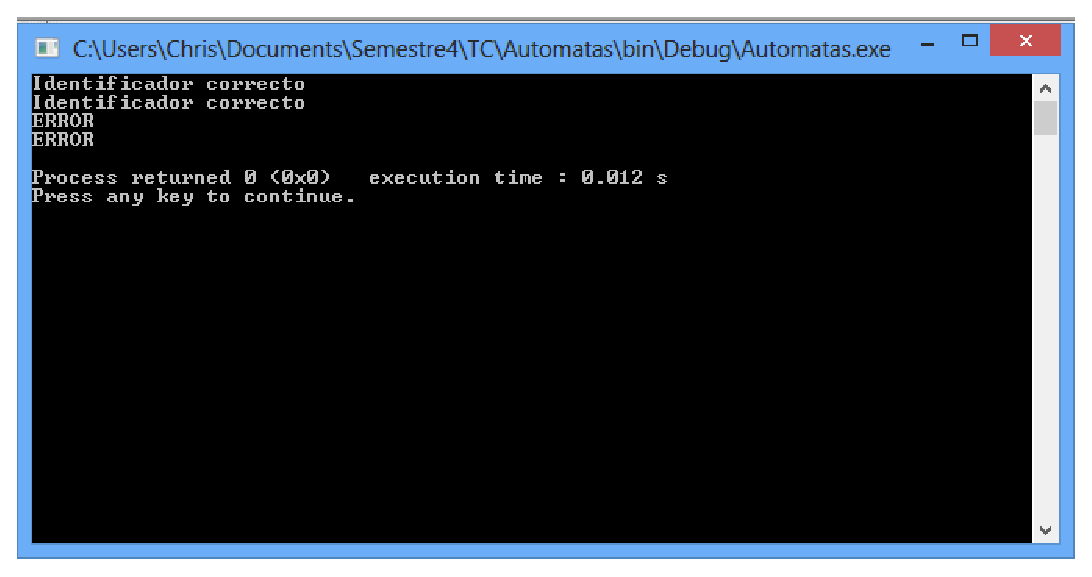
\includegraphics[scale=0.5]{imagenes/1.eps}
\caption{Ejemplo 1}
\end{figure}

\subsection{Verificar Identificador con tabla de Transiciones}

Para este ejemplo usaremos los mismos identificadores del archivo "datos.txt" cuyo contenido se mostro anteriormente.

\begin{figure}[h]
\centering
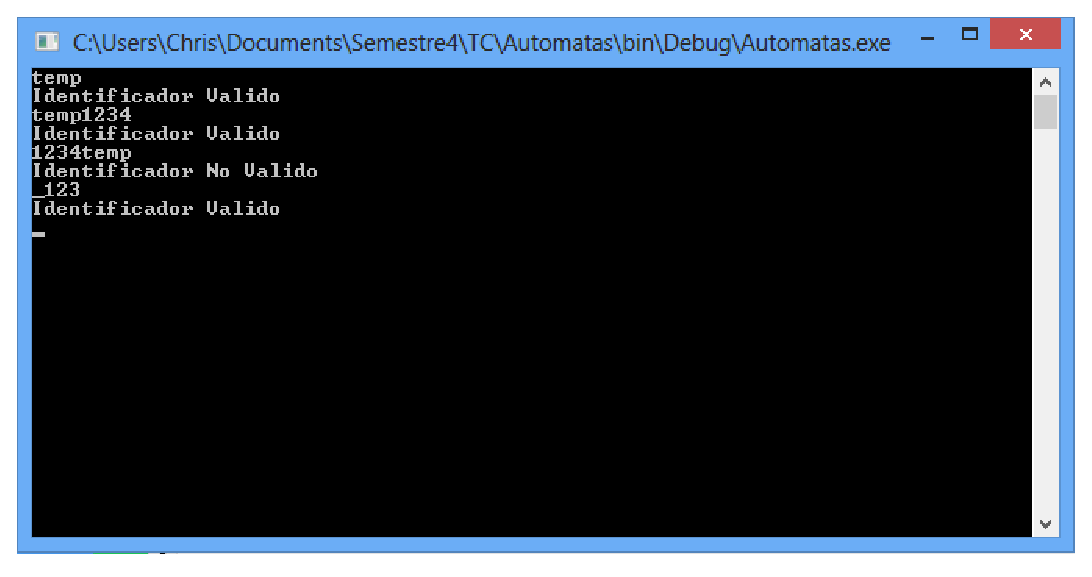
\includegraphics[scale=0.5]{imagenes/2.eps}
\caption{Ejemplo 2}
\end{figure}
\newpage

\subsection{Verificar Número Real con Diagrama de Transiciones}

\begin{figure}[h]
\centering
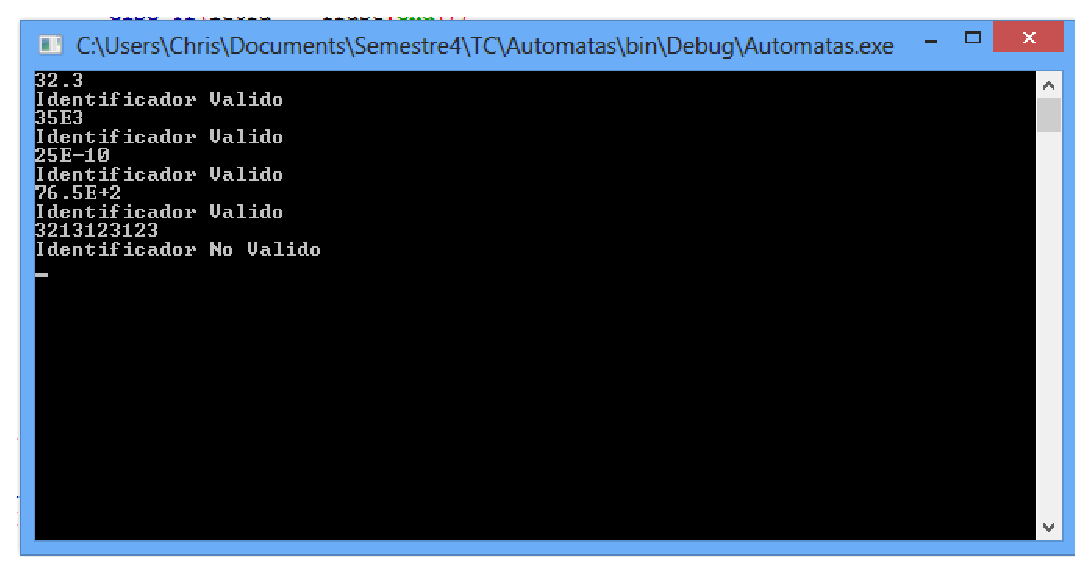
\includegraphics[scale=0.5]{imagenes/3.eps}
\caption{Ejemplo 3}
\end{figure}



\subsection{Verificar Número Real cond Tabla de Transiciones}

\begin{figure}[h]
\centering
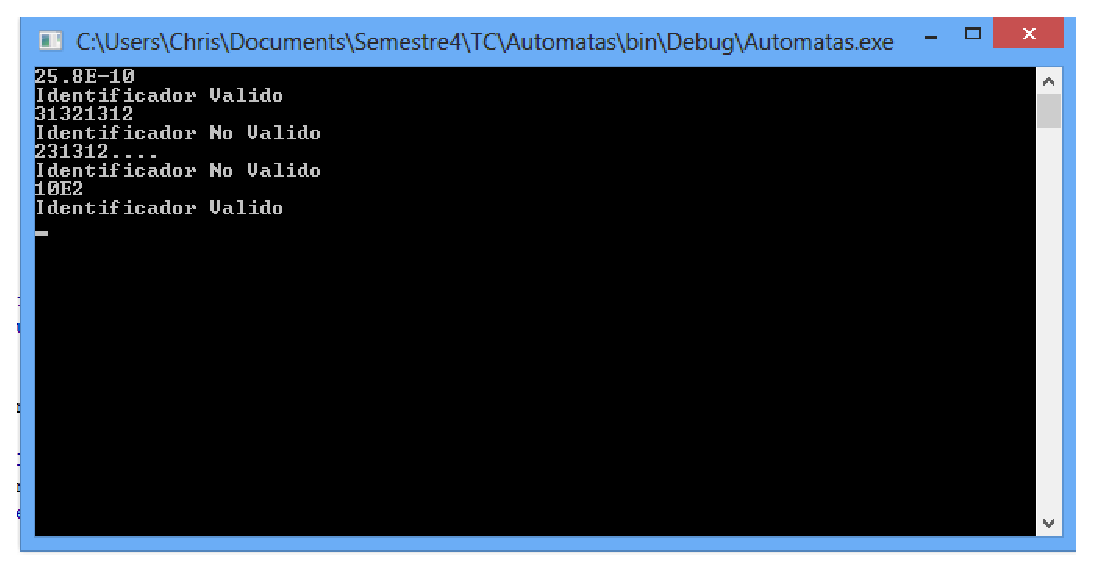
\includegraphics[scale=0.5]{imagenes/4.eps}
\caption{Ejemplo 4}
\end{figure}


\end{document}
